\section{Results}\label{s:evaluation}

\begin{table*}[htbp]
\centering
\small
\caption{ABR performance summary on Mahimahi 4G traces.}
\label{tab:abr_results_4g}
\begin{tabular}{@{\hskip 4pt}l@{\hskip 6pt}r@{\hskip 6pt}r@{\hskip 6pt}r@{\hskip 6pt}r@{\hskip 6pt}r@{\hskip 6pt}r@{\hskip 6pt}r@{\hskip 6pt}r@{\hskip 4pt}}
\toprule
\textbf{ABR} & \textbf{SSIM} & \textbf{Buffer (s)} & \textbf{Rebuffer (s)} & \textbf{RTT (ms)} & \textbf{Delivery Rate (bytes/s)} & \textbf{SSIM Rank} & \textbf{Rebuffer Rank} & \textbf{Buffer Rank} \\
\midrule
BOLA      & 0.97408 & 11.57 & 13.43 & 1{,}050.064 & 814{,}454   & 5 & 6 & 4 \\
Gelato    & 0.97478 & 12.27 &  6.61 &   989.020 & 809{,}936   & 2 & 2 & 5 \\
Linear    & 0.97474 & 11.43 &  6.97 & 1{,}054.478 & 834{,}774   & 3 & 3 & 3 \\
MPC       & 0.97471 & 10.82 & 12.86 & 1{,}086.598 & 819{,}035   & 4 & 5 & 1 \\
Pensieve  & 0.96322 & 14.01 &  6.20 &   639.466 & 742{,}120   & 6 & 1 & 6 \\
TTP       & 0.97533 & 11.18 &  7.82 & 1{,}021.934 & 755{,}283   & 1 & 4 & 2 \\
\bottomrule
\end{tabular}
\end{table*}

\begin{table*}[htbp]
\centering
\small
\caption{ABR performance summary on Mahimahi 5G traces.}
\label{tab:abr_results_mahimahi5g}
\begin{tabular}{@{\hskip 4pt}l@{\hskip 6pt}r@{\hskip 6pt}r@{\hskip 6pt}r@{\hskip 6pt}r@{\hskip 6pt}r@{\hskip 6pt}r@{\hskip 6pt}r@{\hskip 6pt}r@{\hskip 4pt}}
\toprule
\textbf{ABR} & \textbf{SSIM} & \textbf{Buffer (s)} & \textbf{Rebuffer (s)} & \textbf{RTT (ms)} & \textbf{Delivery Rate (bytes/s)} & \textbf{SSIM Rank} & \textbf{Rebuffer Rank} & \textbf{Buffer Rank} \\
\midrule
BOLA      & 0.98276 & 14.65 & 0.279 & 174.018 & 2{,}981{,}315 & 6 & 1 & 3 \\
Gelato    & 0.98391 & 14.65 & 2.014 & 177.588 & 3{,}234{,}831 & 1 & 5 & 5 \\
Linear    & 0.98320 & 14.66 & 0.286 & 177.257 & 3{,}164{,}944 & 4 & 2 & 6 \\
MPC       & 0.98316 & 14.65 & 0.290 & 165.963 & 3{,}124{,}434 & 5 & 3 & 4 \\
Pensieve  & 0.98334 & 14.64 & 2.442 & 175.174 & 3{,}136{,}684 & 2 & 6 & 1 \\
TTP       & 0.98320 & 14.64 & 0.318 & 164.800 & 3{,}037{,}121 & 3 & 4 & 2 \\
\bottomrule
\end{tabular}
\end{table*}

\begin{table*}[htbp]
\centering
\small
\caption{ABR performance summary on CellReplay 5G traces.}
\label{tab:abr_results_cellreplay5g}
\begin{tabular}{@{\hskip 4pt}l@{\hskip 6pt}r@{\hskip 6pt}r@{\hskip 6pt}r@{\hskip 6pt}r@{\hskip 6pt}r@{\hskip 6pt}r@{\hskip 6pt}r@{\hskip 6pt}r@{\hskip 4pt}}
\toprule
\textbf{ABR} & \textbf{SSIM} & \textbf{Buffer (s)} & \textbf{Rebuffer (s)} & \textbf{RTT (ms)} & \textbf{Delivery Rate (bytes/s)} & \textbf{SSIM Rank} & \textbf{Rebuffer Rank} & \textbf{Buffer Rank} \\
\midrule
BOLA      & 0.98277 & 14.67 & 0.181 & 59.930 & 5{,}029{,}392 & 6 & 1 & 6 \\
Gelato    & 0.98392 & 14.66 & 1.818 & 60.406 & 5{,}390{,}346 & 1 & 5 & 3 \\
Linear    & 0.98322 & 14.67 & 0.187 & 60.147 & 5{,}296{,}908 & 4 & 2 & 5 \\
MPC       & 0.98319 & 14.65 & 0.200 & 59.920 & 5{,}164{,}358 & 5 & 3 & 2 \\
Pensieve  & 0.98354 & 14.66 & 2.403 & 61.081 & 5{,}317{,}908 & 2 & 6 & 4 \\
TTP       & 0.98322 & 14.65 & 0.234 & 60.327 & 5{,}129{,}787 & 3 & 4 & 1 \\
\bottomrule
\end{tabular}
\end{table*}

In this section, we evaluate six ABR algorithms: \textit{BOLA}, \textit{Gelato}, \textit{Linear BBA}, \textit{MPC}, \textit{Pensieve}, and \textit{TTP}, across various network conditions and different emulators. We evaluated both application-layer metrics and transport-layer metrics. We report the mean values for each metric, calculated as the average of all values computed per video segment during playback. This gives us an overall performance estimate for the entire test duration. For all experiments, we used the same 10-minute video from the CBS channel that Puffer provides to ensure fair testing for all experiments.

\subsection{4G Traces in Mahimahi}

\begin{figure}[htbp]
    \centering
    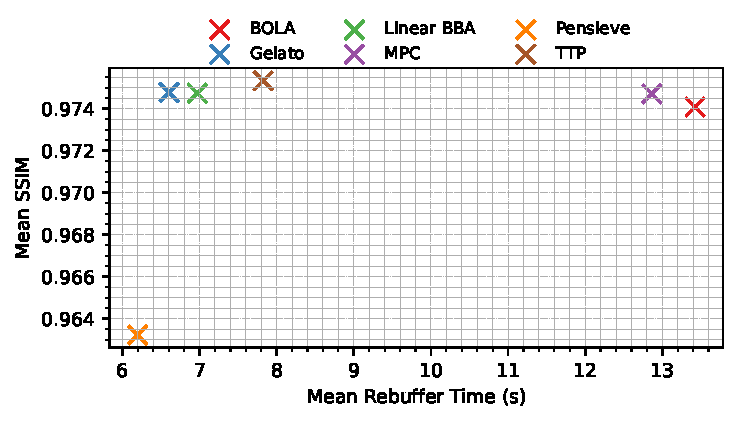
\includegraphics[width=\linewidth]{figs/graphs/ssim_rebuffer_4G}
    \caption{SSIM vs. Rebuffer time for ABR algorithms under Mahimahi 4G traces.}
    \label{fig:ssim_rebuffer_4g}
\end{figure}

We ran experiments using the 4G traces included in Mahimahi’s repository, specifically from AT\&T, T-Mobile, and Verizon. These traces capture real-world mobile conditions and represent networks with limited bandwidth. In this experiment, we observed how ABRs behave in a bandwidth-constrained environment. As demonstrated in Figure~\ref{fig:ssim_rebuffer_4g} and Table~\ref{tab:abr_results_4g}, ABRs show clear differences in multiple metrics. TTP achieves the highest average SSIM around 0.9753 and a middle-ground rebuffering time of 7.82 seconds. 

Pensieve has the lowest rebuffering time around 6.20 seconds, but does not deliver quality as good as other ABRs (with SSIM around 0.9632). This indicates that Pensieve prioritizes stable playback over quality, by down-switching quality to lower rebuffer time, averaging a lower SSIM.

MPC and BOLA struggle the most on 4G. Although they deliver a decent quality, SSIM around 0.9747 and 0.9741, they both average a high rebuffering time around 12.86 and 13.43 seconds, respectively.

Finally, Gelato and Linear BBA offer an average performance among all ABRs. They average SSIM values around 0.9747 and 0.9748, and moderate rebuffer times around 6.61 and 6.97 seconds, respectively.

In summary, Figure~\ref{fig:ssim_rebuffer_4g} shows a better understanding of where each ABR stands. Algorithms on the top left, TTP, Gelato, and Linear BBA tend to maintain a balance between good quality and rebuffering. We can conclude that they offer the best QoE balance in 4G. For other algorithms, the trade-off is between quality and rebuffering.

\subsection{5G Traces in Mahimahi}

\begin{figure}[htbp]
    \centering
    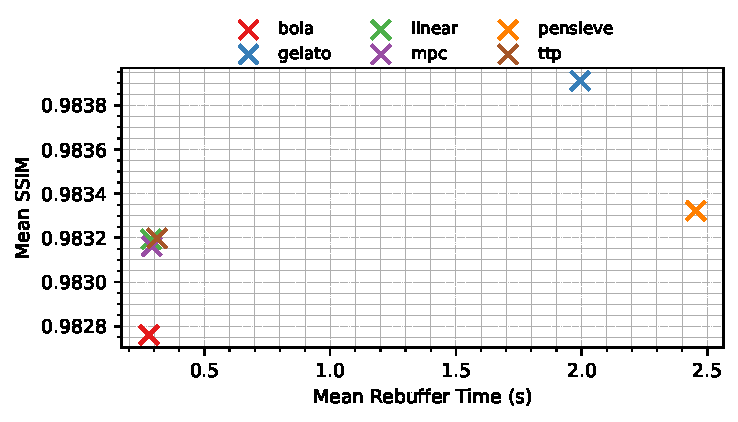
\includegraphics[width=\linewidth]{figs/graphs/ssim_rebuffer_5Gmahimahi}
    \vspace{10pt}
    \caption{SSIM vs. Rebuffer time for ABR algorithms under Mahimahi 5G traces.}
    \label{fig:mahimahi5g}
\end{figure}

With improved network conditions, we used the same 5G traces in both Mahimahi and CellReplay environments to evaluate ABR performance. Using Figure~\ref{fig:mahimahi5g} and Table~\ref{tab:abr_results_mahimahi5g}, our objective is to compare these results to 4G traces, as well as to evaluate how different emulators change the behavior of ABR. All algorithms improved significantly in both quality and stability. The average rebuffer times drop to around 0.3 to 2.5 seconds, which shows that the capacity of 5G significantly affects the average rebuffer time for every ABR. In particular, BOLA and MPC have averaged around 0.28 to 0.29 seconds of rebuffer time, ranking as the best in rebuffer time under 5G, whereas on 4G they were ranked the worst. Their improvement shows that the stalling was likely due to limited bandwidth. They also serve a higher quality (SSIM around 0.9828 and 0.9831). This indicates that with sufficient bandwidth, BOLA and MPC can achieve stable and reasonably high-quality playback.

On the other hand, Gelato achieves the highest SSIM around 0.9839 among all ABRs, but with around 2 seconds of rebuffering. This suggests that Gelato pushes for the highest-quality playback while experiencing some stalls. 

Pensieve also serves the second highest quality with SSIM around 0.9833, but stalls more than other algorithms, with around 2.44 seconds of rebuffering. Interestingly, in 4G scenarios, Pensieve achieved the most stable playback with around 6.20 seconds of rebuffering, while providing the lowest quality, whereas in 5G it is the other way around. This suggests that Pensieve is less cautious than other algorithms in high-throughput networks.

TTP and Linear BBA maintain an average rebuffer time of under approximately 0.3 seconds in this environment, with a reasonably high SSIM (above 0.983). These algorithms can be considered as more stable choices along with MPC and BOLA, due to their balanced performance.

Overall, the results of 5G in the Mahimahi environment show that higher bandwidth levels play a crucial role in delivering high-quality and stable playback. All algorithms deliver nearly the same top quality, so the real differentiator here is how successful each algorithm is in avoiding minor stalls.

\subsection{5G Traces in CellReplay}

\begin{figure}[htbp]
    \centering
    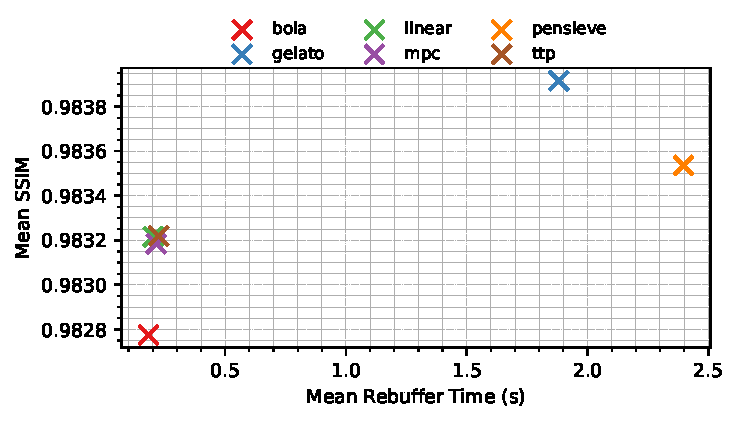
\includegraphics[width=\linewidth]{figs/graphs/ssim_rebuffer_5GCellreplay}
    \caption{SSIM vs. Rebuffer time for ABR algorithms under CellReplay 5G traces.}
    \label{fig:cellreplay5g}
\end{figure}

We tested the same 5G traces using CellReplay as an emulator and observed similar high performance trends, Figure~\ref{fig:cellreplay5g} and Table~\ref{tab:abr_results_cellreplay5g}, with a few noticeable differences compared to Mahimahi. All ABRs achieved close SSIM values around 0.982-0.984. The increase in video quality and lower rebuffer time is negligible but still present. Under 5G conditions, all algorithms are capable of delivering top-quality playback.

Gelato maintains the highest SSIM around 0.9839 also in CellReplay. It still has the second-highest rebuffering around 1.82 seconds. 

BOLA, Linear BBA, and MPC manage to keep their rebuffer times under 0.2 seconds, again slightly lower than the experiment in Mahimahi, with a minor improvement in the SSIM range (around 0.9827-0.9832).

TTP also maintains a low rebuffer of around 0.23 seconds. These results confirm that most ABRs perform similarly well in sufficient bandwidth.

Pensieve is mostly affected by the quality, while other algorithms improved more on rebuffering time. When we compare Figures~\ref{fig:mahimahi5g} and~\ref{fig:cellreplay5g}, we observe that while most algorithms shift noticeably to the left, Pensieve shows minimal horizontal movement. However, it experiences the largest vertical movement in SSIM, suggesting improved quality in CellReplay.

In general, both emulators remain consistent when the same traces are used in terms of video quality and rebuffer time. But improved results suggest that CellReplay's more advanced design gives algorithms more headroom to operate in, providing better quality switches.

\subsection{Emulator Comparison: Mahimahi vs. CellReplay}

A key part of our evaluation involves directly comparing the differences between the two emulators, Mahimahi and CellReplay, using the same 5G traces. This helps us to understand how CellReplay differs from Mahimahi as an emulation tool, since it was built as a slightly more advanced version of Mahimahi, aiming to overcome some of its known limitations.

Inspecting Table~\ref{tab:abr_results_mahimahi5g} and Table~\ref{tab:abr_results_cellreplay5g}, we can make direct comparisons of the overall results. The biggest difference is seen in RTT and delivery rate. CellReplay maintains an average RTT around 55–60 milliseconds, which is close to the real 5G latency. Mahimahi's RTT is much higher, often over 140 milliseconds, due to its simplified delay model, which introduces artificial delays.

We also observe a consistent gap between the two emulators in terms of delivery rate. CellReplay offers higher throughput, with average delivery rates reaching up to 5.3 million bytes per second, while Mahimahi reaches up to 3.2 million. The advanced design of CellReplay better reflects the nature of 5G traffic than Mahimahi. As a result, this gives ABR algorithms more room to operate, leading to decisions such as higher quality selections, fewer quality switches, and overall improved playback with less stalling.

Lower latency and higher throughput affect how ABRs behave. Although the changes are not very large, we still observe some impact on rebuffering and video quality. When feedback is delayed, ABRs become more cautious, which can result in slightly more rebuffering and slower adaptation. For example, Pensieve showed a smaller rebuffering gap between Mahimahi and CellReplay. Gelato, on the other hand, improved more noticeably in CellReplay. This shows that all algorithms are influenced by network conditions, but the extent of that impact depends on how each ABR reacts to changes in throughput and delay.

\begin{figure}[htbp]
    \centering
    \begin{subfigure}[t]{\linewidth}
        
\includegraphics[width=\linewidth]{graphs/buffer_barchart_mahimahi5G}
        \caption{Mahimahi 5G}
        \label{fig:buffer-barchart-mahimahi5G}
    \end{subfigure}
    \vspace{1em}

    \begin{subfigure}[t]{\linewidth}
        
\includegraphics[width=\linewidth]{graphs/buffer_barchart_cellreplay5G}
        \caption{CellReplay 5G}
        \label{fig:buffer-barchart-cellreplay5G}
    \end{subfigure}

    \caption{Mean buffer time across ABR algorithms under Mahimahi and CellReplay using 5G traces. The figure illustrates the average buffer occupancy (in seconds) for each ABR algorithm.}
    \label{fig:buffer-barchart}
\end{figure}

Figure~\ref{fig:buffer-barchart} provides a direct comparison of the mean buffer occupancy between the two emulators. Most algorithms average around 14.6 seconds of video buffer, but their rankings have small shifts when a different emulator is used.

In Mahimahi, Pensieve has the lowest average buffer time, followed by TTP and BOLA, whereas Linear BBA holds the highest among all algorithms. In CellReplay, MPC ranks lowest in buffer time, followed by TTP and Gelato, with BOLA ranking as the highest.

These ranking changes illustrate how the buffer strategies of each algorithm interact with the emulator design. Mahimahi's inflated delay seems to slightly compress buffer occupancy in general, while CellReplay's realistic model allows for subtle differences in how each ABR maintains its buffer under 5G conditions. Most ABRs maintain similar buffer levels across both emulators. However, the slight variations in buffer occupancy reflect each ABR's balance between preloading data and reacting to changing network feedback.

In summary, our comparison shows that the choice of emulator matters in some aspects. Algorithms perform more accurately when realistic network dynamics are used. While Mahimahi might introduce artifacts that can affect ABR behavior, CellReplay offers better control and more realistic results.

\subsection{Trace-Level Variability}

Figures~\ref{fig:rtt-overtime-cellreplay} and ~\ref{fig:rtt-overtime-mahimahi} show RTT differences under different traces (stationary vs. driving) for both emulators. This section focuses on how RTT and Delivery Rate change across traces and networks.

In stationary 5G scenarios, both emulators maintain a lower and more stable RTT over time. In stationary conditions, CellReplay preserves tightly around 40-60 milliseconds, which reflects realistic 5G latencies, where Mahimahi on average holds RTTs over 100 milliseconds, with high peaks in some points. Under these conditions, algorithms behave almost similarly in CellReplay, whereas in Mahimahi, some ABRs like MPC and Linear BBA have peaks around 400 milliseconds across the timeline. 

However, in driving scenarios, both CellReplay and Mahimahi suffer from constant high peaks with an increase in overall RTT. These patterns suggest that mobile and fluctuating traces raise the difficulty of ABR by reducing the consistency of RTT. Algorithms like Gelato, that rely on tight feedback loops, tend to stall and oscillate more under these conditions, whereas other algorithms like MPC and TTP have a more stable performance.

Furthermore, when moving from 4G to 5G, we can see much more significant differences in RTT and delivery rates. When we look at Tables~\ref{tab:abr_results_4g} and~\ref{tab:abr_results_mahimahi5g}, in both metrics, a massive improvement can be seen. In 4G, while average RTTs hover around 1000 milliseconds, this is much lower in 5G, around 164-177 milliseconds. On the other hand, we observe the same differences across delivery rates. 5G traces provide around three times higher throughput compared to 4G traces. As a result, throughput-driven algorithms can benefit more from this increased capacity. In terms of both metrics, these lower values also explain how ABR algorithms provide a better video quality while avoiding more stalls in 5G compared to 4G. 

In conclusion, beyond variations in emulator choice, trace variation is also a key factor, affecting how ABRs behave. It is crucial to design algorithms that adapt not only to bandwidth but also to RTT stability. ABRs with stronger RTT handling perform better in dynamic traces. Therefore, it is important to test algorithms under various realistic trace patterns to find their true characteristics.

\vspace{1em}
\begin{figure*}[htbp]
    \centering
    \begin{subfigure}[t]{3.48in}
        
\includegraphics[width=3.48in, height=2.14in]{graphs/rtt_overtime_tmobile_cellreplay_stationary}
        \caption{T-Mobile CellReplay Stationary}
        \label{fig:rtt-overtime-tmobile-stationary}
    \end{subfigure}
    \hfill
    \begin{subfigure}[t]{3.48in}
        
\includegraphics[width=3.48in, height=2.14in]{graphs/rtt_overtime_tmobile_cellreplay_driving}
        \caption{T-Mobile CellReplay Driving}
        \label{fig:rtt-overtime-tmobile-driving}
    \end{subfigure}
    \caption{RTT over time for ABRs under T-Mobile CellReplay (5G) traces in stationary and driving scenarios.}
    \label{fig:rtt-overtime-cellreplay}
\end{figure*}

\vspace{1em}
\begin{figure*}[htbp]
    \centering
    \begin{subfigure}[t]{3.52in}
        
\includegraphics[width=3.52in, height=2.14in]{graphs/rtt_overtime_tmobile_mahimahi_stationary}
        \caption{T-Mobile Mahimahi Stationary}
        \label{fig:rtt-overtime-tmobile-mahimahi-stationary}
    \end{subfigure}
    \hfill
    \begin{subfigure}[t]{3.31in}
        
\includegraphics[width=3.31in, height=2.14in]{graphs/rtt_overtime_tmobile_mahimahi_driving}
        \caption{T-Mobile Mahimahi Driving}
        \label{fig:rtt-overtime-tmobile-mahimahi-driving}
    \end{subfigure}
    \caption{RTT over time for ABRs under T-Mobile Mahimahi (5G) traces in stationary and driving scenarios.}
    \label{fig:rtt-overtime-mahimahi}
\end{figure*}

\subsection{Transport-Layer Analysis for Networks and Emulators}
\label{sec:tcp-analysis}

We capture all TCP packets during playback and process them using tshark filters to calculate the average number of retransmissions, total packets sent, and retransmission percentage for each ABR algorithm, in different settings. Tables~\ref{tab:tcp-5g-cellreplay},~\ref{tab:tcp-5g-mahimahi}, and~\ref{tab:tcp-4g} display these results in three environments. In both 5G settings, average retransmissions are significantly lower, ranging from 1 to 4 packets per run, or below 0.002\%, compared to 4G traces, where these values go up to 45 to 130 packets per run, or over 0.025\% minimum. For example, BOLA averages only 2 to 2.5 retransmitted packets in 5G, but this value goes up to over 130 packets in 4G settings. Similar trends apply to other algorithms, but not as severe as BOLA, with approximately 45 to 67 retransmissions on average. Higher retransmission rates display poor link quality, where packets drop due to congestion, signal quality, and jitter. This network instability puts more stress on ABR algorithms, forcing them to react by switching quality. This also suggests that algorithms with higher retransmission rates, like BOLA, are more vulnerable to packet loss, causing them to make more aggressive decisions to maintain playback. Another eye-catching result from the tables is the average packets exchanged during playback, and there is a gap between 4G and 5G traces. The lower packet captures suggest that less data were successfully streamed. This can be due to increased rebuffering and more frequent quality down-switching, potentially causing ABR algorithms to make conservative decisions under poor network conditions. Higher retransmission rates cause delays, slowing down the stream, and resulting in fewer packet exchanges within 10 minutes. It is also worth mentioning that the difference is not only in 4G and 5G environments, but the choice of emulator also plays a role. Even though the results are not too far apart between Mahimahi and CellReplay, we can observe the same consistent behavior where CellReplay outperforms Mahimahi, just like in previous evaluations. CellReplay's more advanced latency modeling, stable and lower RTT values, cause fewer retransmissions and more packet exchange on average.

Figures~\ref{fig:retrans-gap-cellreplay}, \ref{fig:retrans-gap-mahimahi}, and ~\ref{fig:retrans-gap-mahimahi4G}, show the time gap between successive retransmissions, \emph{first} and \emph{second}, for each run in different environments. For 5G results, we observed fewer than 2 retransmissions in most runs, unlike 4G traces. In general, 4G traces have higher retransmission rates, and as illustrated from the histograms, they also have frequent retransmissions. Successive retransmissions usually occur immediately, but in some cases they occur between 10 to 70 seconds. This trend changes in 5G traces. In CellReplay, the histogram shows a tight cluster, and every gap falls below 150 seconds, but many traces are collected under 60 to 75 seconds. This behavior with short gaps mimics real 5G fading, where losses come in small bursts, but since the retransmission rates are very low or none in most cases, this suggests that stalling is not as frequent. Mahimahi delivers infrequent, but isolated losses for baseline testing, but is less stressful for congestion control. Successive retransmissions are spread over 0 to 500 seconds.

\begin{table}[t!]
\centering
\small
\caption{Average TCP retransmissions and total packets across \textbf{5G} traces in CellReplay for each ABR algorithm.}
\label{tab:tcp-5g-cellreplay}
\begin{tabular}{@{\hskip 6pt}l@{\hskip 6pt}r@{\hskip 6pt}r@{\hskip 6pt}r@{\hskip 6pt}}
\toprule
\textbf{ABR} & \textbf{Avg Retransmission} & \textbf{Total Packets} & \textbf{Retransmission \%} \\
\midrule
BOLA      & 2.00   & 238{,}397   & 0.000839 \\
Gelato    & 1.75   & 249{,}807   & 0.000700 \\
LinearBBA & 0.75   & 248{,}004   & 0.000302 \\
MPC       & 2.25   & 238{,}480   & 0.000940 \\
Pensieve  & 1.50   & 251{,}827   & 0.000593 \\
TTP       & 1.50   & 238{,}240   & 0.000625 \\
\bottomrule
\end{tabular}
\end{table}

\begin{table}[t!]
\centering
\small
\caption{Average TCP retransmissions and total packets across \textbf{5G} traces in Mahimahi for each ABR algorithm.}
\label{tab:tcp-5g-mahimahi}
\begin{tabular}{@{\hskip 6pt}l@{\hskip 6pt}r@{\hskip 6pt}r@{\hskip 6pt}r@{\hskip 6pt}}
\toprule
\textbf{ABR} & \textbf{Avg Retransmission} & \textbf{Total Packets} & \textbf{Retransmission \%} \\
\midrule
BOLA      & 2.50   & 222{,}277   & 0.001086 \\
Gelato    & 3.00   & 233{,}326   & 0.001244 \\
LinearBBA & 2.00   & 231{,}356   & 0.000839 \\
MPC       & 2.25   & 223{,}014   & 0.000971 \\
Pensieve  & 4.50  & 232{,}681   & 0.001889 \\
TTP       & 2.00   & 222{,}836   & 0.000880 \\
\bottomrule
\end{tabular}
\end{table}

\begin{table}[t!]
\centering
\small
\caption{Average TCP retransmissions and total packets across all \textbf{4G} traces in Mahimahi for each ABR algorithm.}
\label{tab:tcp-4g}
\begin{tabular}{@{\hskip 6pt}l@{\hskip 6pt}r@{\hskip 6pt}r@{\hskip 6pt}r@{\hskip 6pt}}
\toprule
\textbf{ABR} & \textbf{Avg Retransmission} & \textbf{Total Packets} & \textbf{Retransmission \%} \\
\midrule
BOLA      & 131.667  & 170{,}638.333   & 0.143533 \\
Gelato    & 49.333   & 171{,}837.667   & 0.029096 \\
LinearBBA & 53.000   & 181{,}782.333   & 0.030106 \\
MPC       & 45.000   & 173{,}200.333   & 0.025491 \\
Pensieve  & 67.667   & 147{,}693.000   & 0.074226 \\
TTP       & 49.667   & 179{,}226.000   & 0.029802 \\
\bottomrule
\end{tabular}
\end{table}


\vspace{1em}

\begin{figure}[htbp]
\centering
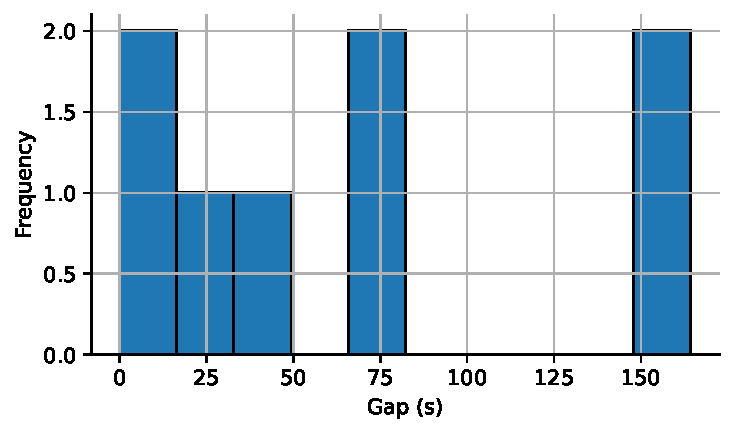
\includegraphics[width=0.83\linewidth]{paper-thesis-fmt/figs/graphs/retransmission_histogram_cellreplay.pdf}
\caption{First successive retransmission time-gap distribution for 5G traces in CellReplay.}
\label{fig:retrans-gap-cellreplay}
\end{figure}

\begin{figure}[htbp]
\centering
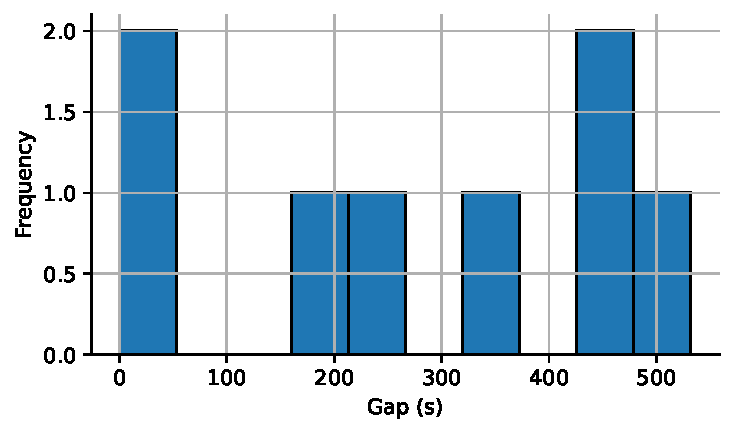
\includegraphics[width=0.83\linewidth]{paper-thesis-fmt/figs/graphs/retransmission_histogram_mahimahi.pdf}
\caption{First successive retransmission time-gap distribution for 5G traces in Mahimahi.}
\label{fig:retrans-gap-mahimahi}
\end{figure}

\begin{figure}[htbp]
\centering
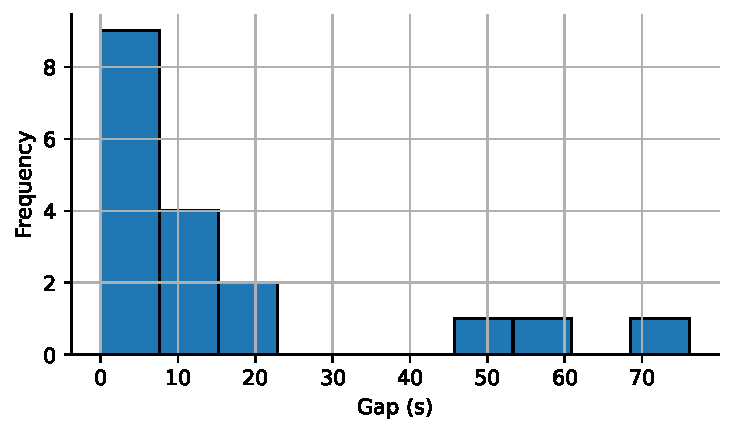
\includegraphics[width=0.83\linewidth]{paper-thesis-fmt/figs/graphs/retransmission_gap_4g.pdf}
\caption{First successive retransmission time-gap distribution for 4G traces in Mahimahi.}
\label{fig:retrans-gap-mahimahi4G}
\end{figure}

\subsection{Overall Comparison}

Tables~\ref{tab:abr_results_4g},~\ref{tab:abr_results_mahimahi5g}, and~\ref{tab:abr_results_cellreplay5g} give the overall mean of each metric and the ranks of each ABR in three different experiments. For each ABR, we can conclude several patterns that we observe from these comparisons;

\begin{itemize}
    \item \textbf{Gelato} consistently delivers the best overall SSIM. In 5G scenarios, it is the leading algorithm and in 4G scenarios, it is the second-best in terms of quality. Although it prioritizes video quality, it sacrifices some overall rebuffering time.
    
    \item \textbf{Pensieve} avoids rebuffering more than others when it comes to challenging network conditions. However, in both 5G scenarios, Pensieve experienced longer rebuffering times. This indicates that Pensieve is sensitive to trace variability. When it comes to slower networks, like 4G, it aggressively reduces quality to prevent stalls. On the other hand, it becomes less cautious in faster networks, like 5G.
    
    \item \textbf{Linear BBA}, \textbf{MPC}, and \textbf{TTP} are mostly balanced in all experiments, providing good overall quality. On 5G traces, for both Mahimahi and CellReplay, all algorithms have had relatively low rebuffering. Linear BBA and TTP performed quite well in 4G, showing reliability and adaptability. However, although MPC pushes to achieve decent quality, it tends to stall more on 4G networks, making it less reliable than TTP and Linear BBA.
    
    \item \textbf{BOLA} offers the lowest quality in almost every scenario, but has lower rebuffer time compared to other algorithms in 5G scenarios. In 4G, it stalls more than any other algorithm. BOLA prioritizes stability over quality compared to other algorithms in faster networks but does not offer the same performance in slower ones.
\end{itemize}

More importantly, these results demonstrate that no ABR algorithm can be universally considered as the best. Depending on the network conditions and user needs, a different ABR may be preferred.

%%% Local Variables:
%%% mode: latex
%%% TeX-master: "../thesis"
%%% End:
